\documentclass{beamer}
\usepackage{graphicx,float}
\usetheme{Median}

\title{\Huge Welcome to GRiD!}
\author{Kostis}
\date{Fall '14}

\begin{document}
\frame{
\maketitle}

\frame{
\frametitle{You may wonder what is the topic of this group...}

\pause 
... after all \textit{data science} is a very broad field. 


\begin{figure}[h]
\centering
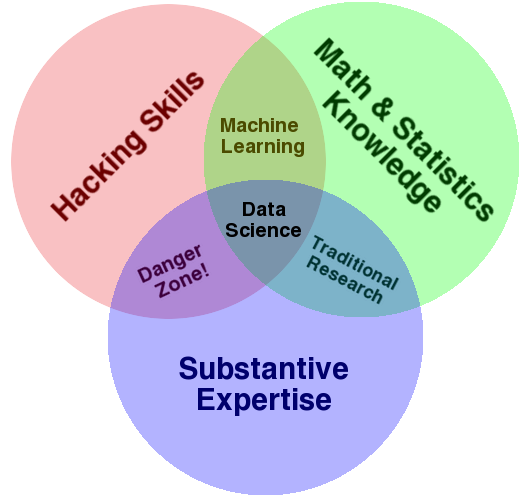
\includegraphics[width=0.45\textwidth]{data_science.png}
\caption{"stolen" from wikipedia data science page.}
\end{figure}
}

\frame{
	\frametitle{What is off-limits?}
	\pause
	\textbf{Absolutely nothing}, in so far as it's relevant.
	
	\pause
	\medskip
	
	Possible topics could be : 
	\begin{itemize}
	\item<1-> Regression techniques (linear and generalized).
	\item<1-> Uncertainty Quantification.
	\item<1-> Data Parsing and clean-up.  
	\item<1-> Machine learning (supervised/unsupervised).
	\item<1-> Data visualization (python, R, processing, javascript, etc). 
	\item<1-> Statistical tools. 
	\pause
	\item<2-> And anything else that {\Large\textbf{you}} think could be interesting.
	\end{itemize}
}

\frame{
	\frametitle{A proposal for our meetings.}
	
	1/3 Learning, 2/3 "Playing". 
	
	\begin{enumerate}
	\item<1-> First 20-30 mins : Someone presents a tool/idea/dataset that they are interested in. (If you think it's gonna be something hardcore, send us a reference a bit earlier.)
	\item<2-> Rest of the time : Depends. If it's something we can use on what we are currently doing, then we can play with the new idea. Otherwise, we continue with our usual project. 
	\end{enumerate}

}

\frame{
	\frametitle{Project??}
	
	\begin{itemize}
	\item<1-> Ideally, we will be able to play with a couple of datasets every semester. 
	\item<2-> We should be dataset \textbf{agnostic}!
	\item<3-> Our goal will be to work with the datasets to answer specific questions. Working with different types of datasets will expose us to different problems.  
	\item<4-> Source of datasets : {\Large\textbf{You!}} {\tiny(But also kaggle and our advisors and supporters.)}
	\end{itemize}	
}

\frame{
	\frametitle{Technicalities}
	What do you think of the mailing list? 
	
	\pause
	\medskip
	
	We are a github organization! Send me an e-mail at kgourgou@umass.edu to add you.
	
	
}


\end{document}